\documentclass[border=2pt,tikz]{standalone}



\usetikzlibrary{decorations.pathmorphing}
\begin{document}
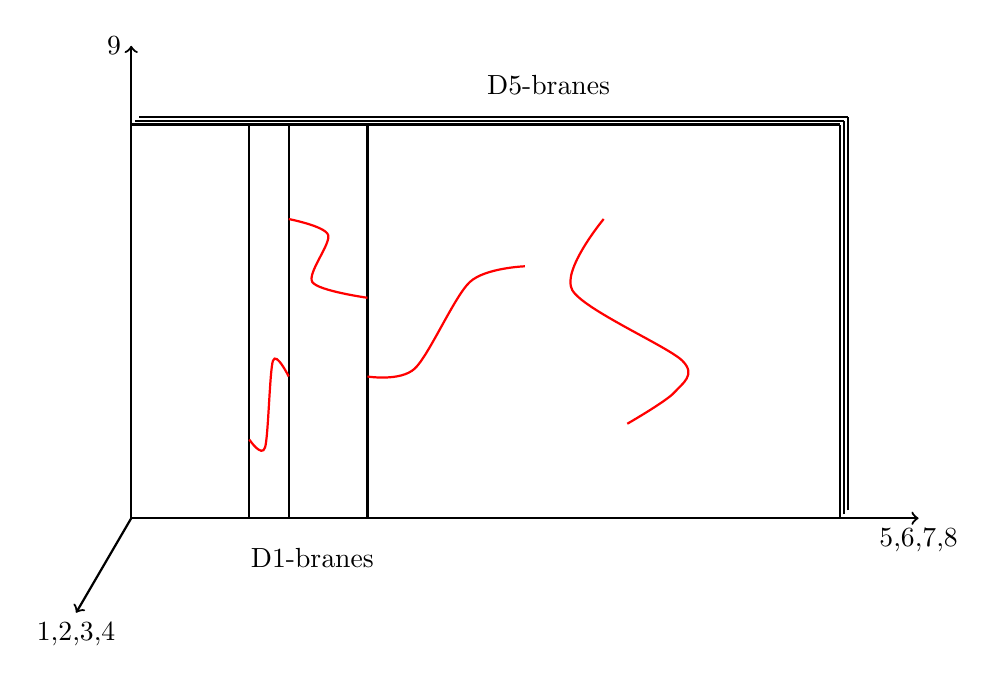
\begin{tikzpicture}[remember picture]
\draw[->,thick] (0,0) -- (0,6) node[left] {9};
\draw[->,thick] (0,0) -- (10,0) node[below] {5,6,7,8};
\draw[->,thick] (0,0) -- (-.7,-1.2) node [below] {1,2,3,4};
\draw[thick] (0,5) -- (9,5) ;
\draw[thick] (0.1,5.1) -- (9.1,5.1);
\draw[thick] (0.05,5.05) -- (9.05,5.05);
\draw[thick] (9,0) -- (9,5) ;
\draw[thick] (9.05,0.05) -- (9.05,5.05) ;
\draw[thick] (9.1,0.1) -- (9.1,5.1) ;
\draw[thick] (3,0) -- (3,5) ;
\draw[thick] (2,0) -- (2,5) ;
\draw[thick] (1.5,0) -- (1.5,5) ;
\draw[thick,red] plot [smooth] coordinates {(1.5,1) (1.7,.9) (1.8,2)  (2,1.8)};
\draw[thick,red] plot [smooth] coordinates {(2,3.8) (2.5,3.6) (2.3,3)  (3,2.8)};

\draw[thick,red] plot [smooth] coordinates {(3,1.8) (3.6,1.9) (4.3,3)  (5,3.2)};
\draw[thick,red] plot [smooth] coordinates {(6,3.8) (5.6,2.9) (7,2) (6.9,1.6)  (6.3,1.2)};

\node at (2.3,-.5) {D1-branes};
\node at (5.3,5.5) {D5-branes};
\end{tikzpicture}
\end{document}